% !TeX root = ../yuwen-book.tex
\chapter{宋代风雪}

% https://www.chinawriter.com.cn/n1/2019/0430/c418957-31059174.html

\vspace{0.4cm}

\begin{center}
\Large\bfseries 宋代风雪\\[0.25em]
{\small\color{black!55} 结构梳理与写法批注}
\end{center}

\vspace{0.3cm}

\begin{handoutlayout}

\section*{逐段解析（1--5）}

\begin{enumerate}[leftmargin=*,label=\protect\circnum{\arabic*},labelsep=0.8em,itemsep=0.9em]

\item 想到宋代，首先想起的是一场场大雪，想到宋太祖雪夜访赵普，想到程门立雪，想到林教头风雪山神庙，仿佛宋代，总有着下不完的雪。

\item 张择端的《清明上河图》，也是从隆冬画起的。枯木寒林中，一队驴子驮炭而行，似乎预示着今夜有暴风雪。萧瑟的气氛，让宋朝的春天显得那么遥远和虚幻。

\item 《水浒传》也可以被看作描绘宋代的绘画长卷。《水浒传》里，令我印象最深的文字是关于雪的。文字随着那份寒冷，深入我的骨髓。《水浒传》里的大雪是这样的：“（那时）正是严冬天气，彤云密布，朔风渐起，却早纷纷扬扬卷下一天大雪来。”还写：“（林冲）带了钥匙，信步投东。雪地里踏着碎琼乱玉，迤逦背着北风而行。那雪正下得紧。”

\item 大雪，在林冲的世界里纷纷扬扬地落着，好像下了一个世纪，下满了整个宋代，严严实实地封住了林冲的去路。

\item 林冲身为八十万禁军枪棒教头，其实是没有任何实权的底层公务员，所以高衙内才会对他百般加害。但即使如此，林冲想的还是逆来顺受，一心想在草料场好好改造，争取早日重返社会，与家人团聚。只是陆虞候不给他出路，高俅不给他出路，留给他的路只有一条，那就是“反”。逼上梁山，重点在一个“逼”字，没有奸臣逼他，林冲一辈子都上不了梁山。连林冲这样一个尿人都反了，《水浒传》对那个时代的批判，是何等的不留情面。

\end{enumerate}

\switchcolumn

\section*{讲义提要}

\begin{structurebox}
\subsection*{1--2：起笔定调}
\begin{itemize}[leftmargin=*]
    \item 第 1 段连用典故起笔，迅速拉出宋代风雪的文化背景；
    \item 第 2 段转入《清明上河图》，用隆冬萧瑟继续压低全文色调。
\end{itemize}
\end{structurebox}

\begin{summarybox}
\subsection*{3--5：由雪写人，由人写世}
\begin{itemize}[leftmargin=*]
    \item 第 3 段从《水浒传》切入，把“雪”与社会压迫、人心之冷联结起来；
    \item 第 4 段把个人命运放大到整个宋代，悲剧感骤然加重；
    \item 第 5 段继续深挖“逼上梁山”的逻辑，完成对黑暗现实的批判。
\end{itemize}
\end{summarybox}
\begin{techbox}
\subsection*{写法批注}
\begin{itemize}[leftmargin=*]
    \item `【作用】` 用典故引出宋代总有下不完的雪，给全文奠定深沉、冷寂的基调；
    \item `【作用】` 从《清明上河图》解读出隆冬的萧瑟，进一步巩固冷寂基调；
    \item `【作用】` 从文学入手，用林冲遭遇把“雪”和“社会压迫”“人心之冷”紧密结合；
    \item `【解读】` 将林冲的个人命运与整个时代的大雪联系起来，强化无力感和悲剧色彩；
    \item `【写法】` 个人感受 + 原文引用 + 深入分析，逐层推进批判力度。
\end{itemize}
\end{techbox}

\begin{keyquote}
大雪下满整个宋代，也封住了林冲的去路。
\end{keyquote}

\end{handoutlayout}

\newpage

\begin{handoutlayout}

\section*{逐段解析（6--10）}

\begin{enumerate}[leftmargin=*,label=\protect\circnum{\arabic*},labelsep=0.8em,itemsep=0.9em]
\setcounter{enumi}{5}

\item 那才是真正的冷，是盘踞在人心里、永远也焐不热的冷。宋徽宗画《祥龙石图》、画《瑞鹤图》，那“祥”“瑞”，那热烈，都被林冲这样一个小角色，轻而易举地颠覆了。

\item 宋代的人都没有读过《水浒传》，但一入宋代，中国绘画就呈现出大雪凝寒的气象。像郭熙的《关山春雪图》、范宽的《雪山萧寺图》等，都是以雪为主题的名画。雪，突然成了宋代绘画的关键词。以至到了明代，画家刘俊仍然以一幅描述赵匡胤雪夜访赵普的《雪夜访普图》，向这个朝代致敬。

\item 这在以前的绘画中是不多见的。晋唐绘画，色调明媚而雅丽，万物葱茏，光影婆娑，与绢的质感相吻合，有一种丝滑流动的气质。

\item 到了宋代，绘画分了两极——一方面，有黄荃、黄居寀、崔白、苏汉臣、李嵩、张择端、宋徽宗等，以花鸟、人物、风俗画的形式描绘他们眼中的世界，田间草虫、溪边野花、林中文士、天上飞鹤，无不凸显这个朝代的繁荣与华美；另一方面，又有那么多的画家痴迷于画雪，画繁华落尽、千峰寒色的寂寥幽远，画“淮南皓月冷千山，冥冥归去无人管”的浩大意境，画“一片白茫茫大地真干净”的清旷虚无，这似乎预示了北宋时代的鼎盛繁华，最终都将指向靖康元年的那场大雪。

\item 宋代雪图中的清旷冷寂、肃杀，确实有气候变化的原因。艺术史与气候史，有时就是一枚硬币的两面。

\end{enumerate}

\switchcolumn

\section*{右栏批注}

\begin{structurebox}
\subsection*{6--8：由文学转入绘画}
\begin{itemize}[leftmargin=*]
    \item 第 6 段先把“雪”从景物推进到人心之冷；
    \item 第 7 段转向宋代雪图，打开艺术史维度；
    \item 第 8 段用晋唐与宋代的对比，为后文“时代气象”蓄势。
\end{itemize}
\end{structurebox}

\begin{summarybox}
\subsection*{9--10：由美术史推进到气候史}
\begin{itemize}[leftmargin=*]
    \item 第 9 段提出关键判断，把艺术与自然并置；
    \item 第 10 段再从宋代扩展到历史周期，完成“点、面、深”的三级推进。
\end{itemize}
\end{summarybox}

\begin{techbox}
\subsection*{批注汇总}
\begin{itemize}[leftmargin=*]
    \item `【修辞】` 拟人，把物理上的寒冷转化成心理感受；
    \item `【结构】` 承上启下，让“林冲之冷”自然过渡到“宋画之冷”；
    \item `【作用】` 转向艺术，指出宋代绘画中雪主题的兴盛；
    \item `【对比】` 用晋唐绘画与宋代绘画对照，突出时代气象差异；
    \item `【写法】` 排比推进，写出宋代由盛转衰的宿命感；
    \item `【写作积累】` 用“艺术史与气候史”建立跨领域的新视角。
\end{itemize}
\end{techbox}

\begin{keyquote}
艺术史与气候史，有时就是一枚硬币的两面。
\end{keyquote}

\end{handoutlayout}

\newpage

\begin{handoutlayout}

\section*{逐段解析（11--14）}

\begin{enumerate}[leftmargin=*,label=\protect\circnum{\arabic*},labelsep=0.8em,itemsep=0.9em]
\setcounter{enumi}{10}

\item 隋唐时代，中国气候温暖，所以隋唐绘画，如实地反映了当时的气候状况。那时的中国人，窝在长安城里，吃着肉夹馍，度过了一个又一个暖冬。冬天的气温尚且如此，春夏就更不用说了。我甚至想，唐朝女人衣着暴露——袒胸露背，蝉衣轻盈，气候温暖应当是一个前提条件。世间能有多少人，甘愿为了风度而牺牲温度呢？

\item 宋代中国的气候寒冷，比唐代冷得多。宋代画家用一场场大雪，坐实了那个朝代的冷，以至我们今天面对宋代的雪图时，依然能感到彻骨的寒凉。有学者认为，中国历史上曾经出现过四个寒冷期，分别是：东周、三国两晋南北朝、五代十国两宋、明末清初。而这四个时期，正是群雄逐鹿、血肉横飞、天下乱成一锅粥的时候。那些乱，也可以从气候上找原因，因为中国是以农业立国，老百姓靠天吃饭，气候极寒导致粮食歉收，造成大面积饥馑，加上朝廷腐败等因素，很容易使天下陷入动乱。

\item 宋人画雪，不是天寒地冻的好，而是静思、坚韧的好。假若还有希望，也不是金光大道艳阳天的那种希望，而是置之死地而后生的希望。

\item 我看过莱昂纳多·迪卡普里奥的电影《荒野猎人》，他演的那个脖子被熊抓伤、骨头裸露、腿还瘸了的荒野猎人，就是在无边的雪地里，完成了生命的逆袭。但在几百年前，在中国的《水浒传》里，施耐庵就已经把这样一种寓意，赋予豹子头林冲。于是，在少年时代的某一个夜晚，我躲在温暖的被窝里，读到如许文字：“林冲投东去了两个更次，身上单寒，当不过那冷。在雪地里看时，离的草场远了，只见前面疏林深处，树木交杂，远远的数间草屋，被雪压着，破壁缝里透出火光来……”

\item 我相信在宋徽宗的晚年，他所有的眼泪都已流完，所有的不平之气都已经消泯，他只是一个白发苍苍的普通老头，话语中融合了河南和东北两种口音，在雪地上执拗地生存着。假若他那时仍会画画，真该画一幅《雪江归棹图》，在生命的最后时刻，对自己颠沛的一生，做一个交代。

\end{enumerate}

\switchcolumn

\section*{右栏批注}

\begin{structurebox}
\subsection*{11：主题升华}
\begin{itemize}[leftmargin=*]
    \item 第 11 段是主旨句最集中的位置；
    \item 文章在这里把“冷”转换成“静思、坚韧、希望”；
    \item 全文情绪由压抑转向有力量的托举。
\end{itemize}
\end{structurebox}

\begin{summarybox}
\subsection*{12--13：对照展开}
\begin{itemize}[leftmargin=*]
    \item 第 12 段用《荒野猎人》与《水浒传》做中外对照；
    \item 第 13 段用“实”的文学与“虚”的想象做虚实对照；
    \item 两组对照都服务于“绝境中的坚韧”这一核心主题。
\end{itemize}
\end{summarybox}

\begin{techbox}
\subsection*{批注汇总}
\begin{itemize}[leftmargin=*]
    \item `【写法】` 观点 + 具体表现 + 学者观点 + 关联社会本质；
    \item `【层次】` 从宋代之冷写到历史周期，再写到社会动荡的因果链；
    \item `【作用】` 将“画雪”升华为静思、坚韧和置之死地而后生的希望；
    \item `【写法——中外对照】` 用《荒野猎人》与《水浒传》印证“绝境中的坚韧”；
    \item `【写法——文学与想象对照】` 用一实一虚延续全文的文学余味；
    \item `【口音的用意】` 借河南与东北两种口音，写宋徽宗在屈辱中仍保有自我。
\end{itemize}
\end{techbox}

\begin{keyquote}
\teachmark{宋人画雪，不是天寒地冻的好，而是静思、坚韧的好。}

首尾呼应：开头以经典典故引出宋代风雪，结尾以宋徽宗的想象场景结束，呼应前文的雪与历史，升华绝境求生的主题。
\end{keyquote}

\end{handoutlayout}

\newpage

\section*{写作手法总结}

\begin{handoutlayout}

\begin{techbox}
\subsection*{一、《水浒传》林冲素材写法}
\begin{itemize}[leftmargin=*]
    \item 个人感受 + 原文引用 + 深入分析；
    \item 从寒冷入骨髓的感受，到书中精彩描写，再到理性分析：百般加害、逆来顺受、没有出路、逼上梁山；
    \item 批判了当时社会的黑暗。
\end{itemize}
\end{techbox}

\begin{techbox}
\subsection*{二、对比手法}
\begin{itemize}[leftmargin=*]
    \item 晋唐绘画：明媚雅丽；
    \item 宋代：一部分画花鸟人物，繁荣华美；一部分画雪，寂寥悠远，预示着靖康之变。
\end{itemize}
\end{techbox}

\begin{techbox}
\subsection*{三、排比}
用“寂寥幽远”“浩大意境”“清旷虚无”三个意象，写出宋代由盛转衰的宿命感。
\end{techbox}

\switchcolumn

\begin{techbox}
\subsection*{四、层次递进}
\begin{itemize}[leftmargin=*]
    \item 点：一段围绕宋代的冷展开，具体表现为宋代画家的大雪；
    \item 面：再拓展至历史周期——引用学者观点，将宋代纳入“四个寒冷期”的历史框架；
    \item 深：关联社会本质——挖掘“寒冷期”与“乱世”的关联，从自然现象延伸到社会动荡。
\end{itemize}
\end{techbox}

\begin{techbox}
\subsection*{五、素材使用}
\begin{itemize}[leftmargin=*]
    \item \textbf{中外对照}：《荒野猎人》与《水浒传》的“雪地逆袭”对照，说明“绝境中的坚韧”是人类共通的精神内核；
    \item \textbf{文学与想象对照}：《水浒传》文字是“实”，宋徽宗画《雪江归棹图》是“虚”，一实一虚中让“雪”成为连接不同人生的精神纽带。
\end{itemize}
\end{techbox}

\begin{keyquote}
这篇文章最值得学习的，不只是素材多，而是素材之间始终围绕“风雪”同向发力。
\end{keyquote}

\end{handoutlayout}


\section*{名画赏析}

\begin{handoutlayout}

此图描写宋太祖赵匡胤雪夜访赵普的历史故事。据《宋史·赵普本传》记载：“太祖数微行过功臣家，普每退朝，不敢便衣冠。一日，大雪问夜，普意帝不出。久之，闻叩门声，普亟出，帝立风雪中，普惶惧迎拜，帝曰：‘已约晋王矣。'已而太宗至，设重裀地坐堂中，炽炭烧肉，普妻行酒，帝以嫂呼之。因与普计下太原。”画面描绘的正是这一历史情景。

在门庭宽敞、屋宇数重的枢密副史府内，前厅正中二人围炉而坐。上首坐的是宋太祖赵匡胤，他头扎巾帽，身穿盘领窄袖袍服，腰束锦带，身材魁伟，气度不凡，其庄严的表情、侧首聆听的姿态，恰当地表现了深夜访贤、商议国家大事的仪态和心境。身着便服的枢密副史赵普在下首侧坐，恭谦地侃侃而谈，细致地刻画出了他诚恳献策的谋臣风度。

画家在着意刻画主体人物的同时，对景象也做了细致描写。近岩远山、老树昏鸦，均被夜色笼罩着，竹叶、树枝、屋脊上覆盖着皑皑白雪，天气显然很寒冷。为突出赵匡胤的天子身份，在大门外象征性地画有四个侍卫，他们似乎守候已久。这些细微的描绘，深化了雪夜访贤的主题。

\switchcolumn

\begin{structurebox}
\subsection*{作品信息}
《雪夜访普图》轴，明，刘俊作，绢本，淡设色，纵 143.2cm，横 75cm。
\end{structurebox}

\begin{center}
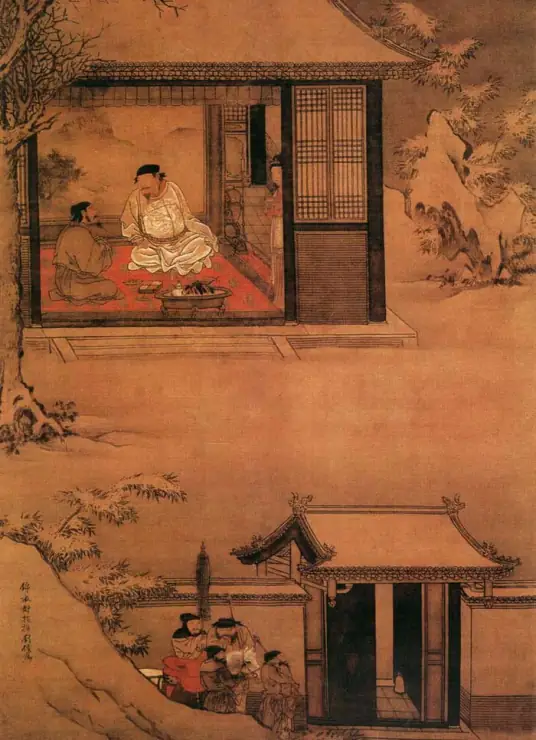
\includegraphics[width=\linewidth]{image/刘俊-雪夜访普图.png}
\end{center}

\begin{summarybox}
\subsection*{图注说明}
\textbf{图名：} 刘俊《雪夜访普图》

\textbf{看点：} 围炉人物、门庭空间、屋脊积雪、门外侍卫。
\end{summarybox}

\begin{techbox}
\subsection*{看图提示}
\begin{itemize}[leftmargin=*]
    \item 先看人物主次：谁居上首，谁在倾听，谁在进言；
    \item 再看环境氛围：雪、夜色、庭院纵深如何烘托“访贤”；
    \item 最后看主题表达：画面如何把历史故事转化为视觉叙事。
\end{itemize}
\end{techbox}

\begin{keyquote}
这幅画最值得关注的，不只是“雪夜访贤”的故事本身，更是人物仪态、庭院层次与雪景气氛如何共同服务主题。
\end{keyquote}

\end{handoutlayout}
